\section{Security}
\begin{frame}{Security Against Bofs}
	\begin{block}{How to secure the stack?}
		\begin{itemize}
			\item Various methods and techniques\ldots
			\item \ldots{}and various consideration.
			\item Which programming languages?
			\item How to deal with legacy code?
			\item Need of automatic protection.
		\end{itemize}
	\end{block}
\end{frame}

\subsection{Programming Languages}
\begin{frame}{Security: Programming Language}
	\begin{block}{Do programming languages automatically protect stack?}
		\begin{description}
			\item[C/C++]these languages don't provide built-int protection, but offer
				\emph{stack-safe} libraries (e.g. $strcpy() \implies strncpy()$).
			\item[Java/.NET/Perl/Python/Ruby/\ldots]all these languages provide an
				automatic array bound check: no need for the programmer to care of it.
		\end{description}
		\begin{itemize}
			\item According to \url{www.tiobe.com} C is the most used Programming Language in 2012.
			\item \alert{Legacy code still exists: it can't be rewritten!}
			\item Operating systems and compiler should offer automatic protections.
		\end{itemize}
	\end{block}
\end{frame}


\subsection{StackGuard}
\begin{frame}{Security: StackGuard (1998)}
	\begin{block}{A patch for gcc}
		\begin{columns}
			\begin{column}{.6\textwidth}
				\begin{itemize}
					\item ``A simple compiler technique that virtually eliminates buffer
						overflow vulnerabilities with only modest performance penalties''
						\cite{stackguard}.
					\item It offers a method for detecting in a portable and efficient way
						changes to the return address.
					\item StackGuard uses a random \emph{canary} word inserted before
						the return address. The callee, before returning, checks if the canary
						word is unaltered.
				\end{itemize}
			\end{column}
			\begin{column}{.4\textwidth}
				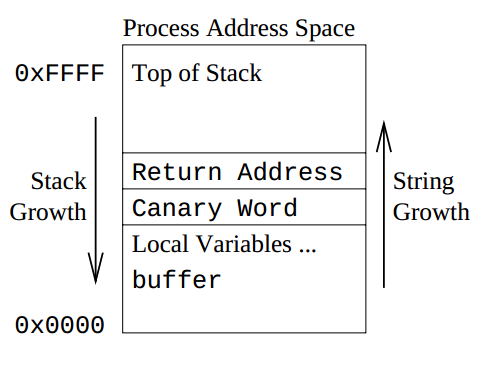
\includegraphics[width=\textwidth]{imgs/sec-canary.png}
			\end{column}
		\end{columns}
	\end{block}
\end{frame}

\subsection{Stack-Smashing Protector}
\begin{frame}{Security: GCC Stack-Smashing Protector (2001)}
	\begin{block}{An improved patch for gcc}
		\begin{columns}
			\begin{column}{.5\textwidth}
		\begin{itemize}
			\item Uses canary word (\textbf{guard}) to protect the base pointer.
			\item Relocate all arrays to the top of the stack in order to prevent variable corruption (\textbf{B} before \textbf{C}).
			\item Copies arguments into new variables below the arrays, preventing argument corruption (\textbf{A} copied into \textbf{C}).
			\item SSP is used by default since gcc 4.0 (2010).
		\end{itemize}
			\end{column}
			\begin{column}{.5\textwidth}
				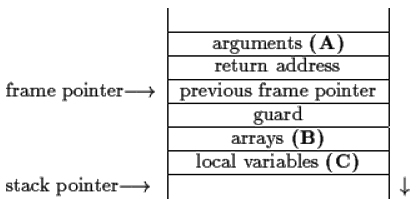
\includegraphics[width=\textwidth]{imgs/sec-ssp.png}
			\end{column}
		\end{columns}
	\end{block}

\end{frame}

\subsection{ASLR}
\begin{frame}[fragile]{Security: Address space layout randomization ($\sim$ 2002)}
	\begin{block}{A runtime kernel protection}
		\begin{itemize}
			\item Using PIC (position independent code) techniques and kernel aid,
				it's possible to change at every execution the position of stack, code
				and library into the addressing space.
			\item Linux implements ASLR since \emph{2.6.12}. Linux ASLR changes the
				stack position.
			\item Windows has ASLR enabled by default since Windows Vista and Windows
				Server 2008. Window ASLR changes stack, heap and Process/Thread
				Environment Block position.
		\end{itemize}
	\end{block}
\end{frame}

\begin{frame}[fragile]{Security: ASLR example}
	\begin{lstlisting}
	# sysctl -w kernel.randomize_va_space=0
	# for i in {1..5}; do ./aslr ; done
		BP: 0x7fffffffe750
		BP: 0x7fffffffe750
		BP: 0x7fffffffe750
		BP: 0x7fffffffe750
		BP: 0x7fffffffe750
	# sysctl -w kernel.randomize_va_space=1
	# for i in {1..5}; do ./aslr ; done
		BP: 0x7fffe03e49d0
		BP: 0x7fff01cd44a0
		BP: 0x7fff23ac2450
		BP: 0x7fffacc72fc0
		BP: 0x7fffa20fca50
	\end{lstlisting}
\end{frame}

\subsection{DEP}
\begin{frame}{Security: Data Execution Prevention ($\sim$ 2004)}
	\begin{block}{Make a virtual page not executable}
		\begin{itemize}
			\item Hardware support using the NX bit (\emph{N}ever e\emph{X}ecute)
				present in modern 64-bit CPUs or 32-bit CPUs with PAE enabled.
			\item NX software emulation techniques for older CPUs.
			\item First implemented on Linux \emph{2.6.8} and on MS Windows since
				\emph{XP SP2} and \emph{Server 2003}.
			\item Currently implemented by all OS (Linux, Mac OS X, iOS, Microsoft Windows and Android).
		\end{itemize}
	\end{block}
\end{frame}

